\section{Dataset Preparation}
\label{sec:data_collection}
\begin{table*}[t]
\center
\begin{tabular}{lccccc}
\toprule[0.2 em]
% \thickhline
Dataset & Real data & Camera pose & 3D map & Video per-frame labeling  & Temporal variations  \\
\hline
\multicolumn{1}{l|}{CamVid~\cite{brostow2009semantic}}     &\checkmark                       & -              & -              &  -  & -  \\
\multicolumn{1}{l|}{KITTI~\cite{geiger2012we}}      &\checkmark  & \checkmark     & sparse points  & -   & -  \\
\multicolumn{1}{l|}{CityScapes~\cite{Cordts2016Cityscapes}} &\checkmark  & -              &  -             & selected frames & - \\
\multicolumn{1}{l|}{Toronto~\cite{wang2016torontocity}}    &\checkmark  & \checkmark     & sparse points  & selected pixels & - \\
\hline
\multicolumn{1}{l|}{Synthia~\cite{RosCVPR16}}    & -          & \checkmark     & -       &\checkmark & -    \\
\multicolumn{1}{l|}{Play for benchmark~\cite{richter2017playing}} &-   & \checkmark     & -     &\checkmark & - \\
\hline
\multicolumn{1}{l|}{Ours}              & \checkmark &\checkmark    &dense point cloud  & \checkmark     &  \checkmark \\
\toprule[0.2 em]
\end{tabular}
\caption{Compare our data with the other related outdoor street-view datasets for our task. 'Real data' mean whether the data is collected from realistic world.
'3D map' means whether it contains 3D map of the whole dataset. 'Video per-frame labeling' means whether it has per-frame per-pixel semantic label.
'Temporal variations' mean whether the recorded video can roughly cover the whole scene, but have multiple. \textcolor[rgb]{1.00,0.00,0.00}{we don't have temporal varations here, we didn't present results on this point neither, that last column needs to be removed. I would also argue the Toronto one is good. 
it has 3D model, so it is dense. In the scope of this paper, we want to paint the picture that 3D maps will be available, so we don't want to over-sell the  uniqueness of our data set.  }}
\label{tbl:data}
\vspace{-0.3\baselineskip}
\end{table*}

\paragraph{Motivation.}
As described in the \secref{sub:framework}, our system is performed with available motion sensors and a semantic 3D map.
However, similar outdoor dataset produced by prior arts such as KITTI and CityScapes, does not containing such information, in particular the 3D map. The Tortoro City dataset~\cite{wang2016torontocity} could be used. However, it is not open yet. As summarized in \tabref{tbl:data}, we list several key properties to perform our experiments.
As can be seen, existing ones that are already open do not satisfy our requirements, especially for pose estimation, 

\textcolor[rgb]{1.00,0.00,0.00}{as I explained in the table, I suggest that we drop this argument, we need to have a 3D semantic map, none has it. the temporal effect needs to be tuned down, otherwise, it will be viewed as too narraow}
for training, we want the recorded video to roughly cover the 3D environment, so that when new images come in, appearance similar views had been seen during training. This means repeated recording at similar spatial locations are required in the data, which we call temporal variations in \tabref{tbl:data}.
However, most existing datasets are a temporal snapshot at some locations in the environment, which requires us to collect a new dataset ourselves.

\paragraph{Data collection.}
We use a mobile LIDAR scanner from $Riegl$ to collect point clouds of the static 3D map with high granularity. As shown in \figref{fig:data}(a). The captured point cloud density is much higher than the Velodyne\footnote{http://www.velodynelidar.com/} used by KITTI~\cite{geiger2012we}.
% Amazingly, it is even able to capture the hight changes of curb on road.
However, different from the sparse Velodyne LIDAR, our mobile scanner utilizes a single laser beam to scan a vertical circle. As the scanner moves, it is able to scan its surroundings as a push-broom camera. It cannot correctly capture moving objects, they will be compressed or expanded or completely missing in the resulting point cloud.
In order to remove those fake object points, thanks to the fact that the 3D world is recorded multiple rounds, and each round has a full coverage of the 3D map, we can use point clouds consistency to handle the issue.
Specifically, we calibrate the 3D point clouds from different rounds, and put all the points together. From the merged point cloud, the points with high temporal consistency from other rounds are kept, while those with low consistency are removed. Formally, the condition to kept a point $\ve{x}$ in round $j$ is,
\begin{align}
\sum_{i=0}^{r}{\mathbbm{1}(\exists~\|\ve{x}_i - \ve{x}_j\| < \epsilon_d )} / r \geq \delta
\end{align}
where $\delta = 0.7$ and $\epsilon_d = 0.025$ in our experiments, and $\mathbb{1}()$ is a indicator function. Notice due to the symmetric property of $\ve{x}_i$ and $\ve{x}_j$, we obtain the static points for all rounds by looping over the points of a single round. We keep the merged point cloud as a static background $\hua{M}$ for further labelling.

For video, we use two cameras facing towards direction of street with a resolution of \by{2048, 2432}, and both cameras are well calibrated \wrt the LIDAR. Based on provided camera parameters from the hardware, all the images from videos are undistorted to match the 3D points.
% talk about registration and removing moving objects inside data

% Undistortion of the image
\paragraph{Label 3D map and videos.}
% talk about labelling in 3D
In order to have semantic labelling of each frame in video, we handle static background, static objects and moving objects separately.
Firstly, for static background, we directly perform labelling on the 3D point cloud $\hua{M}$ which is then projected to images, yielding labelled background for all the frames.
Specifically, we over-segment the point cloud data into point clusters based on spatial distance and normal directions, and then we ask labellers to label each cluster of points manually.
For static objects in each round of video, we prune out the points of static background, and label the remaining points of objects. Due to the fact that when object is static, \eg parked cars, the shape and location of captured points will be highly recognizable, whereas when the object is moving on the road, the points will be fuzzy, we ask labeller to label those can be well recognized as static objects. Last, after projecting the 3D to 2D, only moving objects remain to be labeled. Here, we adopt an active labelling strategy, by first training an object segmentation model using a SOTA algorithm~\cite{WuSH16e}, and ask labellers to correct and label the masks of moving objects.

Finally, as shown in \figref{fig:data}(c), the projected label from 3D points is not perfect, due to missing points either too far away or reflection. We handle such issue by using splatting techniques in computer graphics, that is to turn each point into a small squaure as discussed in \secref{sub:render} (\figref{fig:data}(d)), and then ask labeller to fix missing regions, yielding the final label map (\figref{fig:data}(e)).
With such a strategy, labelling efficiency of video can be vastly increased, avoiding labelling edge rich regions like trees and poles on the street, especially when occlusion is happened.
We provided the labelled video in our supplementary materials for readers who are interested.

\begin{figure}[t]
\begin{center}
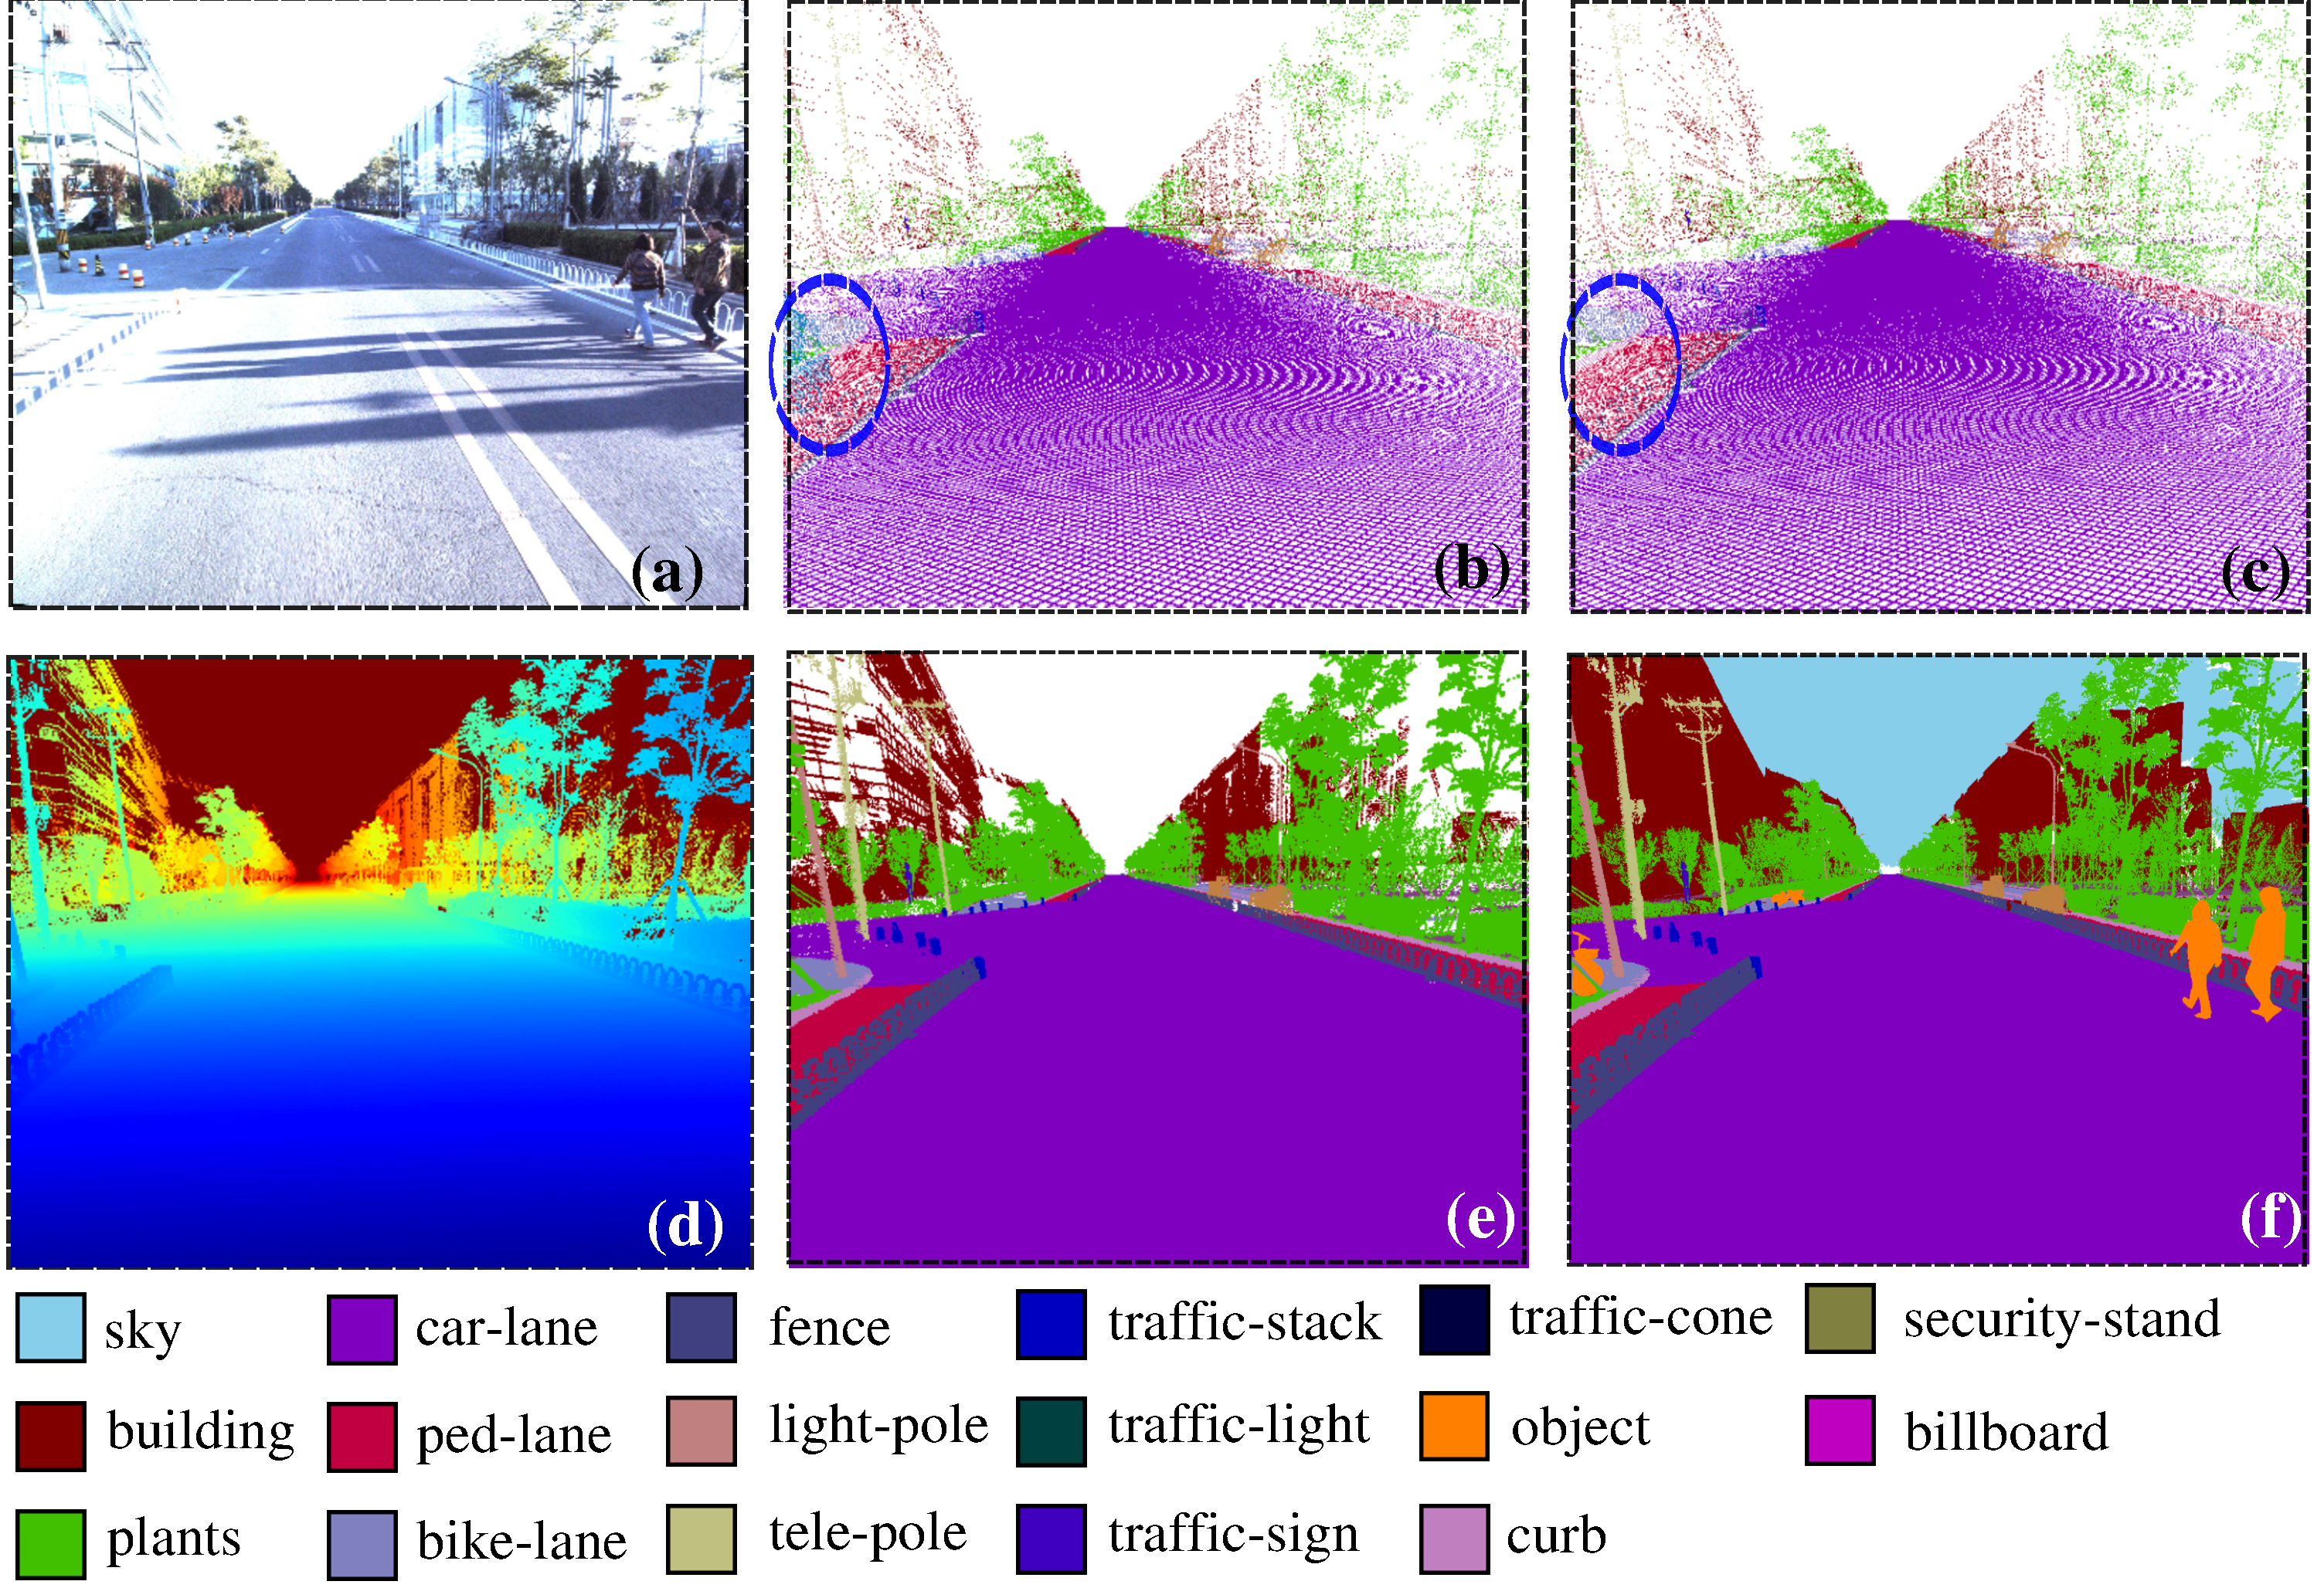
\includegraphics[width=\linewidth]{fig/dataset.pdf}
\end{center}
   \caption{Snapshot of our collected data. (a) 3D semantic map. (b) Images. (c) Rendered label map with 3D points (d) Rendered label map with enlarged square. (e) Merge label map with object and sky.}
\label{fig:data}
\end{figure}
